\documentclass{article}

\usepackage{amsmath,amssymb}
\usepackage{geometry}
\usepackage{graphicx}
\usepackage{booktabs}

\geometry{a4paper, margin=2.5cm}

\begin{document}

% ============================================================
\section*{Temporal-Difference Learning (TD)}

\subsection*{First, a story}

You walk the same route to school every day. Today, halfway there, you find the road closed; the detour costs ten extra minutes. How should you update your prediction of arrival time?

\begin{itemize}
  \item \textbf{Method A}: complete the whole route, look at the clock at home, update your prediction with the actual time. Accurate --- but you must wait until arrival;
  \item \textbf{Method B}: halfway through, glance at the remaining road, estimate today's total, and revise on the spot. No waiting --- but the guess may be biased.
\end{itemize}

Method A is Monte Carlo (MC); method B is \textbf{temporal-difference learning} (TD). TD's core idea: \textbf{don't wait for the outcome} --- after every step, correct the current estimate using ``immediate feedback plus a guess about the future''. You do not need the full truth; one step of feedback and your current prediction suffice.

\subsection*{Formalization: the TD(0) update}

Recall the two extremes:

\textbf{Monte Carlo} --- run the whole trajectory, update with the true return:
\[
V(S_t) \leftarrow V(S_t) + \alpha\bigl[G_t - V(S_t)\bigr], \qquad
G_t = R_{t+1} + \gamma R_{t+2} + \cdots + \gamma^{T-t-1} R_T
\]
$G_t$ is an \textbf{unbiased} estimate of $v_\pi(S_t)$ but has high variance (a whole trajectory fluctuates), and you must wait for the episode to end.

\textbf{Dynamic programming} --- with a known model, take the expectation over all successors:
\[
V(s) \leftarrow \sum_a \pi(a\mid s)\Bigl[R(s,a) + \gamma\sum_{s'} P(s'\mid s,a)\,V(s')\Bigr]
\]
Zero variance, deterministic --- but requires the full model $P(s'\mid s,a)$, rarely available in reality.

\textbf{TD(0)} takes the best of both --- each step uses \textbf{one real reward} and \textbf{the current estimate of the successor}:

\[
\boxed{V(S_t) \leftarrow V(S_t) + \alpha\Bigl[\underbrace{R_{t+1} + \gamma V(S_{t+1})}_{\text{TD target}} - V(S_t)\Bigr]}
\]

\begin{itemize}
  \item $R_{t+1} + \gamma V(S_{t+1})$ --- the \textbf{TD target}: one real reward plus the current estimate of the successor, approximating $G_t$;
  \item $R_{t+1} + \gamma V(S_{t+1}) - V(S_t)$ --- the \textbf{TD error}: the gap between the current estimate and a ``fresher'' one;
  \item vs.\ MC: MC uses the true $G_t$; TD replaces the unknown post-$t{+}1$ rewards with the estimate $V(S_{t+1})$ --- that is \textbf{bootstrapping} (updating an estimate from an estimate);
  \item vs.\ DP: DP's expectation over successors needs $P(s'\mid s,a)$; TD \textbf{samples a single actual} $S_{t+1}$ --- no model required.
\end{itemize}

% ============================================================
\section*{The TD error and the source of ``learning fast''}

\subsection*{A rigorous definition}

At time $t$ the agent is in $S_t$; after acting it receives $R_{t+1}$ and moves to $S_{t+1}$. The TD error is:

\[
\boxed{\delta_t = R_{t+1} + \gamma V(S_{t+1}) - V(S_t)}
\]

If $V = v_\pi$ (the true value function), then $\mathbb{E}[\delta_t \mid S_t=s]=0$ --- an immediate corollary of the Bellman equation:
$v_\pi(s) = \mathbb{E}_\pi[R_{t+1}+\gamma v_\pi(S_{t+1})\mid S_t=s]$. As $V$ approaches $v_\pi$, $\delta_t$ tends to zero mean. TD learning is the process of driving $\delta_t$ toward zero.

\subsection*{MC vs TD(0): the bias--variance trade-off}

\begin{center}
\begin{tabular}{lcc}
\toprule
 & \textbf{MC} & \textbf{TD(0)} \\
\midrule
Update target & $G_t$ (true return) & $R_{t+1}+\gamma V(S_{t+1})$ (one-step estimate) \\
Bootstrapping & no & yes \\
Bias & unbiased & biased \\
Variance & high & low \\
Must wait for episode end & yes & no \\
Needs a model & no & no \\
\bottomrule
\end{tabular}
\end{center}

TD accepts a \textbf{biased} estimate in exchange for \textbf{much lower variance} and faster convergence. On the 5-state random walk (Figure~\ref{fig:td-vs-mc}), both methods consume the same batch of trajectories: MC must average returns with a small step size ($\alpha=0.01$) and lags; TD(0) corrects in place every step with a larger step size ($\alpha=0.1$) and tracks the true values sooner.

\begin{figure}[!htbp]
  \centering
  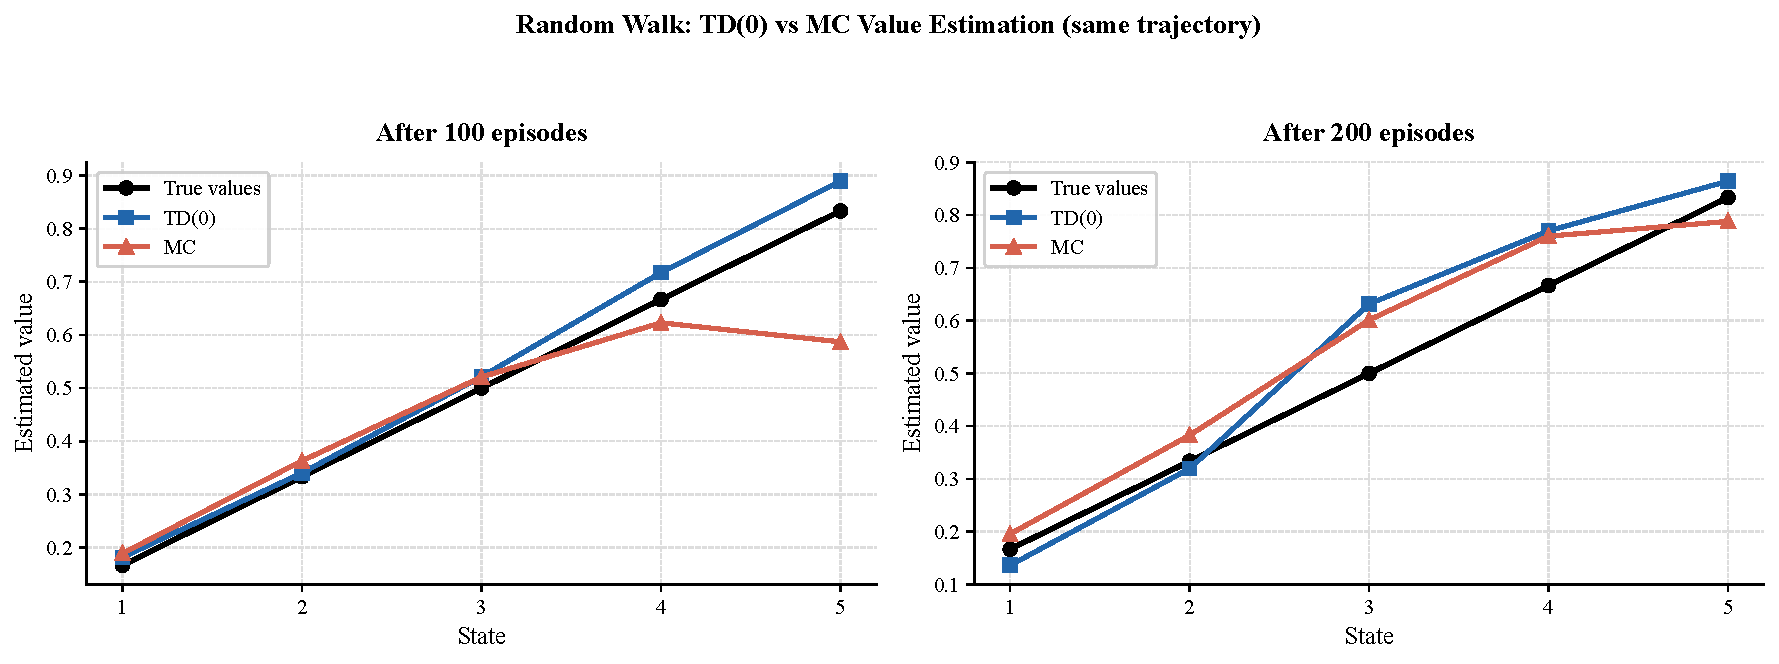
\includegraphics[width=0.85\textwidth]{fig1_random_walk_mc_vs_td.pdf}
  \caption{Value estimates on the 5-state random walk (same batch of trajectories). The black line is the true value $v(s)=s/6$; red is MC ($\alpha=0.01$), blue is TD(0) ($\alpha=0.1$). TD(0) is closer to the truth after both 100 and 200 episodes (100-episode average RMS: MC 0.149 vs TD 0.062).}
  \label{fig:td-vs-mc}
\end{figure}

% ============================================================
\section*{From Prediction to Control: SARSA and Q-Learning}

The previous section used $V$ for prediction; this section uses $Q$ for control (learning a policy).

\subsection*{On-policy: SARSA}

SARSA learns the $q_\pi$ of the policy \textbf{actually executed} (including exploration):

\[
\boxed{Q(S_t,A_t) \leftarrow Q(S_t,A_t) + \alpha\bigl[R_{t+1} + \gamma Q(S_{t+1},A_{t+1}) - Q(S_t,A_t)\bigr]}
\]

Actions are usually chosen by $\varepsilon$-greedy. The SARSA loop:
\begin{enumerate}
  \item in $S_t$, pick $A_t$ $\varepsilon$-greedily;
  \item execute $A_t$, receive $R_{t+1}$, arrive at $S_{t+1}$;
  \item in $S_{t+1}$, \textbf{pick again} $A_{t+1}$ $\varepsilon$-greedily (not executed; only its $Q$ value is used);
  \item update $Q(S_t,A_t)$ with $A_{t+1}$'s $Q$ value;
  \item $S_t \leftarrow S_{t+1}$, $A_t \leftarrow A_{t+1}$, repeat.
\end{enumerate}

The key: $A_{t+1}$ in the target comes from the \textbf{actually executed policy} (with exploration), so SARSA learns the $q_\pi$ of the $\varepsilon$-greedy policy, \textbf{accounting for the cost of exploration}.

\subsection*{Off-policy: Q-Learning}

Q-Learning learns the \textbf{optimal} (greedy) policy while still exploring during execution:

\[
\boxed{Q(S_t,A_t) \leftarrow Q(S_t,A_t) + \alpha\bigl[R_{t+1} + \gamma \max_a Q(S_{t+1},a) - Q(S_t,A_t)\bigr]}
\]

The only difference from SARSA: the target uses $\max_a Q(S_{t+1},a)$ instead of $Q(S_{t+1},A_{t+1})$. SARSA's target depends on the actually sampled $A_{t+1}$ (exploration noise included); Q-Learning's target \textbf{always assumes the best action next}, whatever exploration actually did. Hence off-policy: the \textbf{policy learned} (greedy, optimal) differs from the \textbf{policy executed} ($\varepsilon$-greedy, exploring).

\subsection*{SARSA vs Q-Learning: Cliff Walking}

The classic Cliff Walking environment ($4\times12$ grid, start bottom-left, goal bottom-right; the 10 middle cells of the bottom row are cliff: stepping on one returns to the start with $-100$; ordinary steps cost $-1$) exposes the difference (Figure~\ref{fig:cliff}).

\begin{figure}[!htbp]
  \centering
  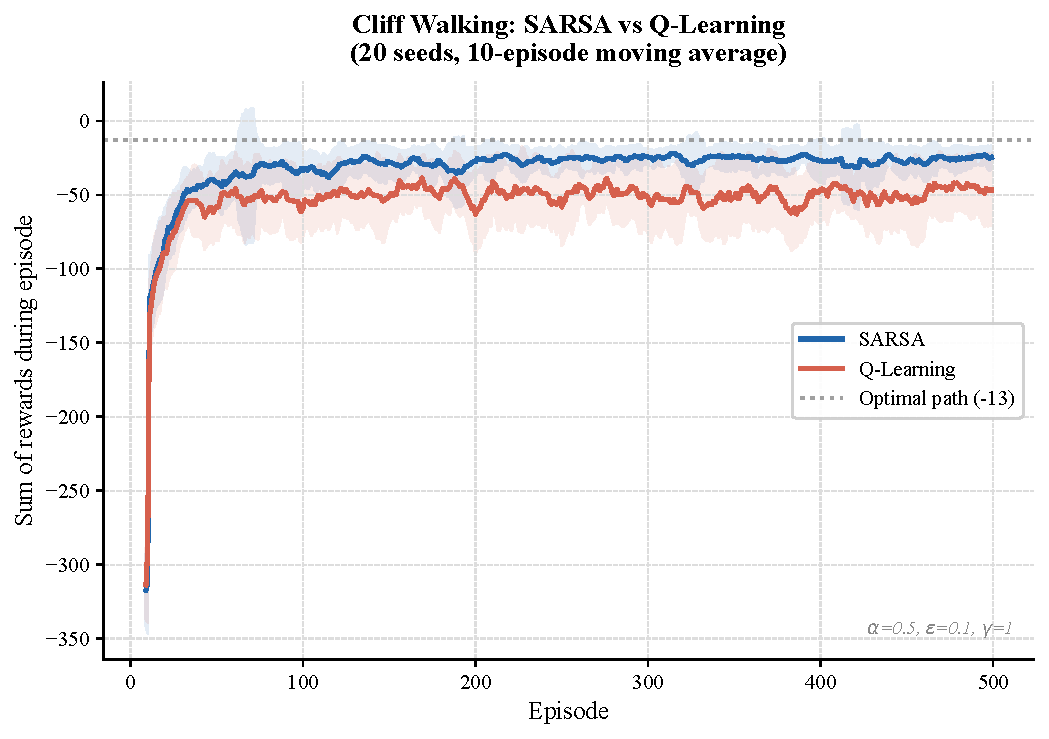
\includegraphics[width=0.85\textwidth]{fig3_cliff_sarsa_vs_qlearning.pdf}
  \caption{Cliff Walking ($4\times12$, $\alpha=0.5$, $\varepsilon=0.1$, $\gamma=1$, 20 random seeds, 10-episode moving average). During training SARSA's per-episode reward is markedly higher: SARSA learns a conservative detour (occasional exploration is not catastrophic), Q-Learning learns the shortest path but repeatedly falls off the cliff during training due to random exploration.}
  \label{fig:cliff}
\end{figure}

\textbf{The key insight}: Q-Learning assumes ``from now on I always act optimally'', so hugging the cliff seems fine (the optimal policy never steps off); SARSA knows that in deployment it will occasionally explore, and one random move along the cliff is a disaster --- hence a safer, more conservative policy. If at deployment the agent is fully greedy ($\varepsilon=0$), Q-Learning's aggressive policy may be better --- it depends on whether your agent can still make mistakes after deployment.

\subsection*{Expected SARSA and the Softmax policy}

\textbf{Expected SARSA} avoids sampling $A_{t+1}$ by taking the expectation over all actions, removing sampling variance:

\[
Q(S_t,A_t) \leftarrow Q(S_t,A_t) + \alpha\Bigl[R_{t+1} + \gamma \sum_a \pi(a\mid S_{t+1})\,Q(S_{t+1},a) - Q(S_t,A_t)\Bigr]
\]

With an $\varepsilon$-greedy target policy it is on-policy; with a purely greedy $\pi$ it \textbf{reduces to Q-Learning} (off-policy). On most tasks Expected SARSA beats plain SARSA --- a tiny compute overhead is repaid many times over by variance reduction.

\textbf{The Softmax policy} distributes exploration probability by relative $Q$ values with temperature $\tau$:

\[
\pi(a\mid s) = \frac{\exp\bigl(Q(s,a)/\tau\bigr)}{\sum_b \exp\bigl(Q(s,b)/\tau\bigr)}
\]

Large $\tau$ approaches uniform exploration; $\tau\to 0$ approaches pure greedy. Exploration is no longer blind ($\varepsilon$-greedy picks every non-greedy action with equal probability $\varepsilon/|\mathcal{A}|$, however obviously bad): \textbf{better actions get more probability}.

% ============================================================
\section*{Multi-step Extensions: n-step TD and TD($\lambda$)}

\subsection*{The n-step return}

TD(0) looks one step ahead (low variance, high bias); MC looks the whole way (unbiased, high variance). \textbf{n-step TD} spans the spectrum; define the n-step return:

\[
\boxed{G_t^{(n)} = R_{t+1} + \gamma R_{t+2} + \cdots + \gamma^{n-1}R_{t+n} + \gamma^n V(S_{t+n})}
\]

\begin{itemize}
  \item $n=1$: $G_t^{(1)} = R_{t+1}+\gamma V(S_{t+1})$ --- TD(0);
  \item $n\to\infty$: $G_t^{(\infty)} = G_t$ --- MC;
  \item $1<n<\infty$: $n$ real rewards, then $V$ estimates the remainder at the truncation point.
\end{itemize}

Update: $V(S_t) \leftarrow V(S_t) + \alpha\bigl[G_t^{(n)} - V(S_t)\bigr]$. n-step SARSA is analogous with $Q$ in place of $V$; replacing the last term by $\sum_a \pi(a\mid S_{t+n})Q(S_{t+n},a)$ gives Expected n-step SARSA.

Figure~\ref{fig:nstep} shows how $n$ moves the bias--variance dial: smaller $n$ (more bootstrapping) yields lower error here; larger $n$ (more real rewards) approaches MC's higher error.

\begin{figure}[!htbp]
  \centering
  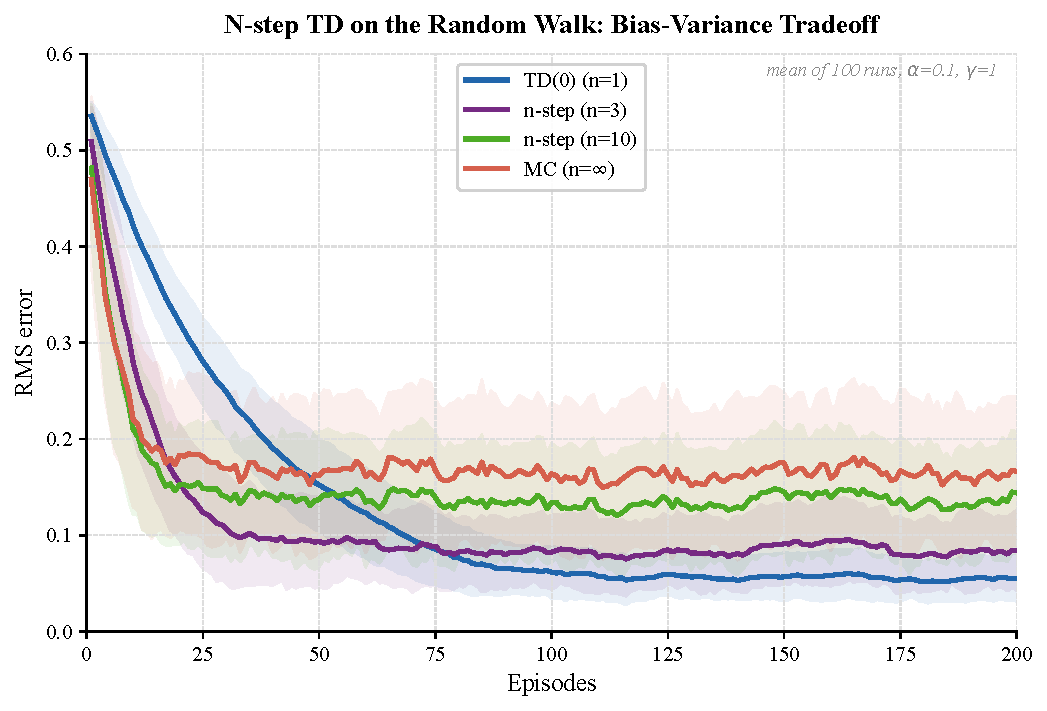
\includegraphics[width=0.85\textwidth]{fig2_nstep_bias_variance.pdf}
  \caption{RMS error of n-step TD on the 5-state random walk vs.\ number of episodes (same $\alpha=0.1$, averaged over 100 episodes). $n=1$ (TD(0)) is lowest; $n=3$ and $n=10$ rise; $n\to\infty$ (MC) is highest --- smaller $n$ bootstraps more, lowers variance, learns faster.}
  \label{fig:nstep}
\end{figure}

\subsection*{TD($\lambda$)}

Rather than a single $n$, TD($\lambda$) mixes all n-step returns with \textbf{geometric weights}:

\[
\boxed{G_t^\lambda = (1-\lambda)\sum_{n=1}^{\infty} \lambda^{n-1} G_t^{(n)}}
\]

\begin{itemize}
  \item $\lambda=0$: $G_t^\lambda = G_t^{(1)}$ --- TD(0);
  \item $\lambda=1$: $G_t^\lambda = G_t$ --- MC;
  \item $0<\lambda<1$: nearer steps get more weight; farther steps contribute less but not zero.
\end{itemize}

$\lambda$ controls the degree of bootstrapping: smaller leans on estimates (high bias, low variance), larger leans on real rewards (low bias, high variance).

\subsection*{Eligibility traces: the online implementation of TD($\lambda$)}

Computing $G_t^\lambda$ requires the whole episode. \textbf{Eligibility traces} give an online incremental form: visiting a state--action pair $(s,a)$ adds $1$ to its trace; every step all traces decay by $\gamma\lambda$:

\[
e_t(s,a) = \begin{cases}
  \gamma\lambda\, e_{t-1}(s,a) + 1, & \text{if } (s,a) \text{ is the current pair}, \\
  \gamma\lambda\, e_{t-1}(s,a),      & \text{otherwise}.
\end{cases}
\]

Update: every step, for all $(s,a)$, $Q(s,a) \leftarrow Q(s,a) + \alpha\,\delta_t\, e(s,a)$. Intuition: the trace is a decaying record of ``how responsible this pair is for the current outcome'' --- recent pairs weigh more, old ones fade to zero.

\textbf{Watkins' Q($\lambda$)}: eligibility traces are naturally on-policy while Q-Learning is off-policy, so special handling is required --- once a non-greedy (exploratory) action is taken, the future trajectory no longer follows the target policy and the traces must be wiped:

\[
\text{if } A_{t+1} \neq \arg\max_a Q(S_{t+1},a) \;\Longrightarrow\; \text{all } e(s,a) \leftarrow 0
\]

The cost: with a high exploration rate, the effective trace length is set by ``the run of consecutive greedy actions'', not by a fixed $\lambda$.

% ============================================================
\section*{Experience Replay --- Data Reuse for Off-Policy}

Online learning uses each transition $(S_t,A_t,R_{t+1},S_{t+1})$ once and discards it --- extremely wasteful. \textbf{Experience replay} maintains a fixed-size buffer of the most recent $N$ transitions:

\begin{enumerate}
  \item the acting policy produces new transitions, stored in the buffer;
  \item a mini-batch is \textbf{sampled uniformly} from the buffer;
  \item multiple Q-Learning updates are performed on the sampled transitions.
\end{enumerate}

Why it works:
\begin{itemize}
  \item \textbf{Breaks correlations}: consecutive transitions are highly correlated; uniform sampling shuffles them, reducing update variance;
  \item \textbf{Sample reuse}: each transition is used multiple times, improving data efficiency;
  \item \textbf{Stabilizes training}: replaying ``old data'' acts as a regularizer.
\end{itemize}

\textbf{Limitation}: experience replay only suits off-policy algorithms (Q-Learning, Expected SARSA). SARSA cannot use it --- its update depends on the current policy's action selection, while buffered data comes from old policies.

% ============================================================
\section*{Where this chapter sits in the RL landscape}

\begin{enumerate}
  \item \textbf{Upstream}: MAB's incremental updates and exploration--exploitation; MDP's Bellman equations and exact DP. DP needs a known model; MC uses true returns (unbiased, high variance, waits for episode end); TD takes the best of both --- one-step sampling plus bootstrapping;
  \item \underline{\textbf{This chapter (TD learning)}}: model-free value learning at its core --- the TD(0) update, the on/off-policy split of SARSA/Q-Learning, n-step and traces tuning the bias--variance dial, and experience replay for off-policy efficiency;
  \item \textbf{Downstream}: Q-Learning's $\max$ operator plus neural-network function approximation equals DQN; replay plus target networks tames the instability of TD updates (next chapter).
\end{enumerate}

\subsection*{The TD algorithm family}

\begin{center}
\begin{tabular}{lcccc}
\toprule
Algorithm & on/off-policy & Bootstrap & Target form & Character \\
\midrule
MC & on & no & $G_t$ & unbiased, high variance \\
TD(0) & on & yes & $R+\gamma V(s')$ & biased, low variance \\
SARSA & on & yes & $R+\gamma Q(s',a')$ & prices in exploration \\
Q-Learning & off & yes & $R+\gamma\max_a Q(s',\cdot)$ & learns the optimum \\
Expected SARSA & both & yes & $R+\gamma\sum_a\pi(a\mid s')Q(s',a)$ & lower variance \\
N-step & both & yes & n-step mixed return & tunable bias--variance \\
Q($\lambda$) & off & yes & $\lambda$-weighted return + traces & online multi-step \\
\bottomrule
\end{tabular}
\end{center}

\begin{itemize}
  \item \textbf{TD(0)}: one real reward plus the next estimate; no waiting for episode end;
  \item \textbf{SARSA}: learn what you execute --- the true $q_\pi$ under $\varepsilon$-greedy, conservative and safe;
  \item \textbf{Q-Learning}: learn $q_*$ directly regardless of exploration;
  \item \textbf{Expected SARSA}: average over the sampled action to cut variance; degenerates to Q-Learning under a greedy $\pi$;
  \item \textbf{N-step TD}: trade bias against variance; larger $n$ approaches MC;
  \item \textbf{TD($\lambda$) + traces}: distribute credit over steps with exponential decay; online multi-step propagation;
  \item \textbf{Experience replay}: store old data, replay uniformly --- decorrelates and improves sample efficiency (off-policy only).
\end{itemize}

\subsection*{The bridge from TD to DQN}

\begin{enumerate}
  \item \textbf{Q-Learning's $\max$ operator + function approximation} = DQN;
  \item \textbf{Experience replay + target networks} = taming the instability of TD updates in DQN;
  \item $\varepsilon$-\textbf{greedy exploration} carries into DQN (simple but effective; later improved by NoisyNet and others);
  \item \textbf{Eligibility traces} $\to$ Retrace-style algorithms $\to$ efficient off-policy multi-step learning with replay.
\end{enumerate}

With this chapter you hold the core of model-free value learning --- TD trades bias for variance via bootstrapping; SARSA/Q-Learning split on/off-policy; n-step and traces tune the dial. The next chapter, DQN, replaces the Q table with a neural network and tames it with replay and target networks.

\subsection*{References}

\begin{enumerate}
  \item Sutton \& Barto (2018). \textit{Reinforcement Learning: An Introduction} (2nd ed.). Chapters 6--7, 12.
  \item Watkins, C.\,J.\,C.\,H. (1989). \textit{Learning from Delayed Rewards}. PhD Thesis. (The original Q-Learning paper.)
  \item Rummery \& Niranjan (1994). On-line Q-learning using connectionist systems. (The original SARSA paper.)
  \item van Seijen et al. (2009). A theoretical and empirical analysis of Expected Sarsa.
  \item Lin (1992). Self-improving reactive agents based on reinforcement learning. (Invention of experience replay.)
  \item Mnih et al. (2015). Human-level control through deep reinforcement learning. \textit{Nature}. (DQN + experience replay.)
  \item Practical RL, Yandex Data School. Week 3 --- Model-Free Reinforcement Learning.
\end{enumerate}

\end{document}
